% This thing is copied from stakcoverflow :P
\documentclass{standalone}

\usepackage{tikz}
\usetikzlibrary{arrows,shapes.geometric,positioning,matrix}
\tikzset{
  ishikawa/.style={align=center, inner sep=0pt},
  matter/.style  ={rectangle, minimum size=6mm, very thick, draw=red!70!black!40,
    top color=white, bottom color=red!50!black!20, font=\itshape},
  level_1/.style ={ellipse, node distance=60pt, minimum size=6mm, very thick,
    draw=red!50!black!50, top color=white, bottom color=red!50!black!20, font=\itshape},
  level_2/.style={rectangle, minimum size=6mm, font=\itshape, font=\scriptsize}}
\tikzset{
  rows/.style 2 args={@/.style={row ##1/.style={#2}},@/.list={#1}},
  cols/.style 2 args={@/.style={column ##1/.style={#2}},@/.list={#1}},
}
\begin{document}
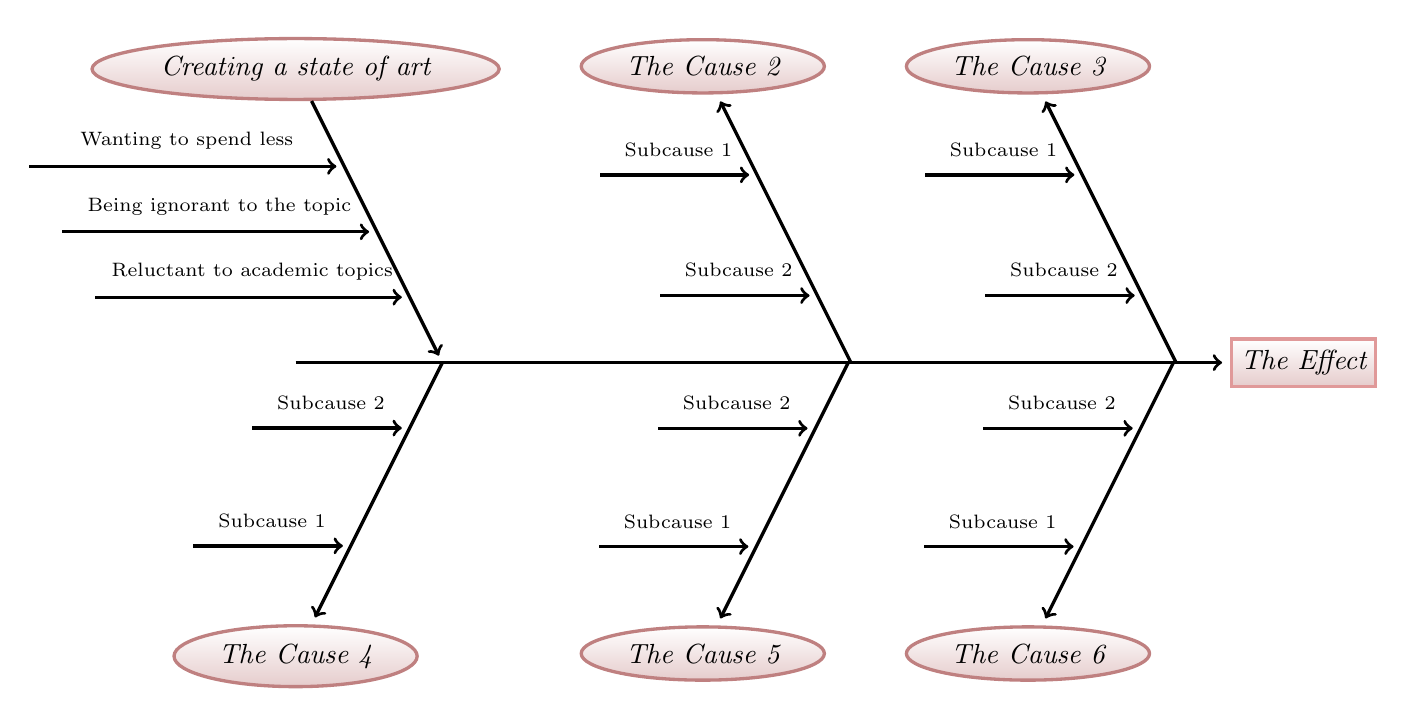
\begin{tikzpicture}
\matrix[
  matrix of nodes,
  row sep=3cm,
  column sep=1cm,
  rows={1,3}{nodes=level_1},
  rows={2}{nodes=matter,anchor=center}
] (m) {
Creating a state of art & The Cause 2 & The Cause 3 & \\
         &         &             & The Effect \\
The Cause 4  & The Cause 5  & The Cause 6     & \\
};
\path[very thick,
  toarr/.style={->, shorten <=+0pt, shorten >=+.1cm},
  fromarr/.style={<-, shorten >=+0pt, shorten <=+.1cm}]

  % Mid left to right arrow
  [toarr]
  (m-1-1|-m-2-4) edge (m-2-4)

  % The Cause 1 arrows
  (m-1-1) edge[xslant=-.5]
    coordinate[pos=.25] (@-1-1-1)
    coordinate[pos=.5]  (@-1-1-2)
    coordinate[pos=.75] (@-1-1-3) (m-1-1|-m-2-4)
  [fromarr]
  (@-1-1-1) edge node[above, align=right, level_2]{Wanting to spend less} ++ (left:4cm)
  (@-1-1-2) edge node[above, align=right, level_2]{Being ignorant to the topic} ++ (left:4cm)
  (@-1-1-3) edge node[above, align=right, level_2]{Reluctant to academic topics} ++ (left:4cm)

  % The Cause 2 arrows
  (m-1-2) edge[xslant=-.5]
    coordinate[pos=.3]   (@-1-2-1)
    coordinate[near end] (@-1-2-2) (m-1-2|-m-2-4)
  [fromarr]
  (@-1-2-1) edge node[above, level_2]{Subcause 1} ++ (left:2cm)
  (@-1-2-2) edge node[above, level_2]{Subcause 2} ++ (left:2cm)

  % The Cause 3 arrows
  (m-1-3) edge[xslant=-.5]
    coordinate[pos=.3]   (@-1-3-1)
    coordinate[near end] (@-1-3-2) (m-1-3|-m-2-4)
  [fromarr]
  (@-1-3-1) edge node[above, level_2]{Subcause 1} ++ (left:2cm)
  (@-1-3-2) edge node[above, level_2]{Subcause 2} ++ (left:2cm)

  % The Cause 4 arrows
  (m-3-1) edge[xslant=.5]
    coordinate[pos=.3]   (@-3-1-1)
    coordinate[near end] (@-3-1-2) (m-3-1|-m-2-4)
  [fromarr]
  (@-3-1-1) edge node[above, level_2]{Subcause 1} ++ (left:2cm)
  (@-3-1-2) edge node[above, level_2]{Subcause 2} ++ (left:2cm)

  % The Cause 5 arrows
  (m-3-2) edge[xslant=.5]
    coordinate[pos=.3]   (@-3-2-1)
    coordinate[near end] (@-3-2-2) (m-3-2|-m-2-4)
  [fromarr]
  (@-3-2-1) edge node[above, level_2]{Subcause 1} ++ (left:2cm)
  (@-3-2-2) edge node[above, level_2]{Subcause 2} ++ (left:2cm)

  % The Cause 6 arrows
  (m-3-3) edge[xslant=.5]
    coordinate[pos=.3]   (@-3-3-1)
    coordinate[near end] (@-3-3-2) (m-3-3|-m-2-4)
  [fromarr]
  (@-3-3-1) edge node[above, level_2]{Subcause 1} ++ (left:2cm)
  (@-3-3-2) edge node[above, level_2]{Subcause 2} ++ (left:2cm);
\end{tikzpicture}
\end{document}

